% cdc.tex
% 
% author : abisutti
% created : Mon, 19 Oct 2015 13:48:21 +0200
% modified : Mon, 19 Oct 2015 13:48:21 +0200



\documentclass{beamer}

\usepackage[T1]{fontenc}
\usepackage[utf8]{inputenc}
\usepackage[francais]{babel}
\usepackage{array}
\usepackage{tabularx}
\usepackage{multirow}
\usepackage{color}
\usepackage{colortbl}
\usepackage{textcomp}
\usepackage{xstring}

%%% MACRO %%%


% FIXME Prendre en compte les majuscule déjà présente
\makeatletter
\@ifpackageloaded{xstring}{
	\newcommand\smallcaps[1]{\StrLeft{#1}{1}\scriptsize\uppercase{\StrGobbleLeft{#1}{1}}\normalsize }
}{
	\newcommand\smallcaps[1]{\textsc{#1}}
}
\makeatother



%===============================================================================
% Définit un type de puce pour une liste. Si le pakage "pifont" est chargé, il 
% est utilisé, sinon on met un tiret.
\makeatletter
\@ifpackageloaded{pifont}{
	\newcommand\goodItemArrow[0]{\ding{226}}
}{
	\newcommand\goodItemArrow[0]{-}
}
\makeatother



%===============================================================================
% Item de liste avec spécification de la puce et paramètre écrit en gras.
\newcommand\functionality[1]{
	\item[\goodItemArrow] \textbf{#1}\\
}



%===============================================================================
% Commande \Euro indépendante des paquets chargés 
\makeatletter
\@ifpackageloaded{eurosym}{
	\newcommand\Euro[0]{\euro{}}
}{
	\@ifpackageloaded{textcomp}{
		\newcommand\Euro[0]{\texteuro}
	}{
		\newcommand\Euro[0]{Euro}
	}
}
\makeatother



%===============================================================================
% Accès à des variables dans le document. 
%\makeatletter
%\let\titleName\@title
%\let\subtitleName\@subtitle
%\let\authorName\@author
%\makeatother



% Titre de la section courante (que dans beamer)
%\secname 
% Titre de la sous-section courante (que dans beamer)
%\subsecname





\title[English Presentation]{Discrete 3D surfaces of revolution}
\subtitle{English Presentation}
\author[]{Zied \smallcaps{Ben} \smallcaps{Othmane} \\ Thomas \smallcaps{Benoist} \\ Adrien \smallcaps{Bisutti} \\ Lydie \smallcaps{Richaume}} % FIXME Enlever les parenthèses
\institute{University of Poitiers}
\date{December 9th of 2015}

\usetheme{Madrid}
\usecolortheme{sidebartab}
\usefonttheme{professionalfonts}
%\useinnertheme{nom du theme interne}
%\useoutertheme{nom du theme externe}



%%% MACRO %%%

% Affichage du plan à chaque début de section
\AtBeginSection[]{
	\begin{frame}{Outline}
		\begin{columns}
			\begin{column}{5cm}
			  	\tableofcontents[sections={1-4}, currentsection, hideothersubsections]
			\end{column}
			\begin{column}{5cm}
			  	\tableofcontents[sections={5-7}, currentsection, hideothersubsections]
			\end{column}
		\end{columns}
	\end{frame}
}

% Nouvelle boîte pour le titre
\definecolor{titlecolor}{RGB}{51, 51, 179}
\newenvironment<>{titleblock}[1]{%
	\setbeamercolor{block body}{fg=white, bg=titlecolor}%
	\begin{block}#2{#1}}{\end{block}}

% Vide la barre de navigation
\setbeamertemplate{navigation symbols}{}

%%% DOCUMENT %%%

\begin{document}


%===============================================================================
%	TITRE
%===============================================================================


\begin{frame}
	\titlepage
	
\includegraphics[width=2cm]{../Images/logo-Xlim.png}
	\hfill
	
\includegraphics[width=2cm]{../Images/logo_univ_poitiers.png}
\end{frame}



%===============================================================================
%	PLAN
%===============================================================================


\begin{frame}{Plan}
	\begin{columns}
		\begin{column}{5cm}
			\tableofcontents[sections={1-4}, hideallsubsections]
		\end{column}
		\begin{column}{5cm}
			\tableofcontents[sections={5-7}, hideallsubsections]
		\end{column}
	\end{columns}
\end{frame}



%===============================================================================
%	INTRODUCTION
%===============================================================================

\section{Introduction}


% --- Équipe -------------------------------------------------------------------
	\subsection{Collaborators and clients}
	\begin{frame}{\subsecname}
		\begin{itemize}
			\item Clients~:
				\begin{itemize}
					\item \'Eric \smallcaps{Andres} (Professor and former director of XLIM-SIC department)
					\item Gaëlle \smallcaps{Largeteau}-\smallcaps{Skapin} (University lecturer, Discrete geometry)
				\end{itemize}
			\item Example of final users~:
				\begin{itemize}
					\item Aur\'elie \smallcaps{Mourier} (Artist)
				\end{itemize}
			\item Pedagogic Supervisor~: 
				\begin{itemize}
					\item Philippe \smallcaps{Meseure} (Professor, Computer Graphics)
				\end{itemize}
		\end{itemize}
	\end{frame}


% --- Contexte -----------------------------------------------------------------
	\subsection{Context}
	\begin{frame}{\subsecname}
		\begin{itemize}
			\item \'Eric \smallcaps{Andres} and Gaëlle \smallcaps{Largeteau}-\smallcaps{Skapin} developped a new algorithm to model discrete surfaces of revolution.
			\item Display the result with Mathematica
		\end{itemize}
		\begin{figure}
			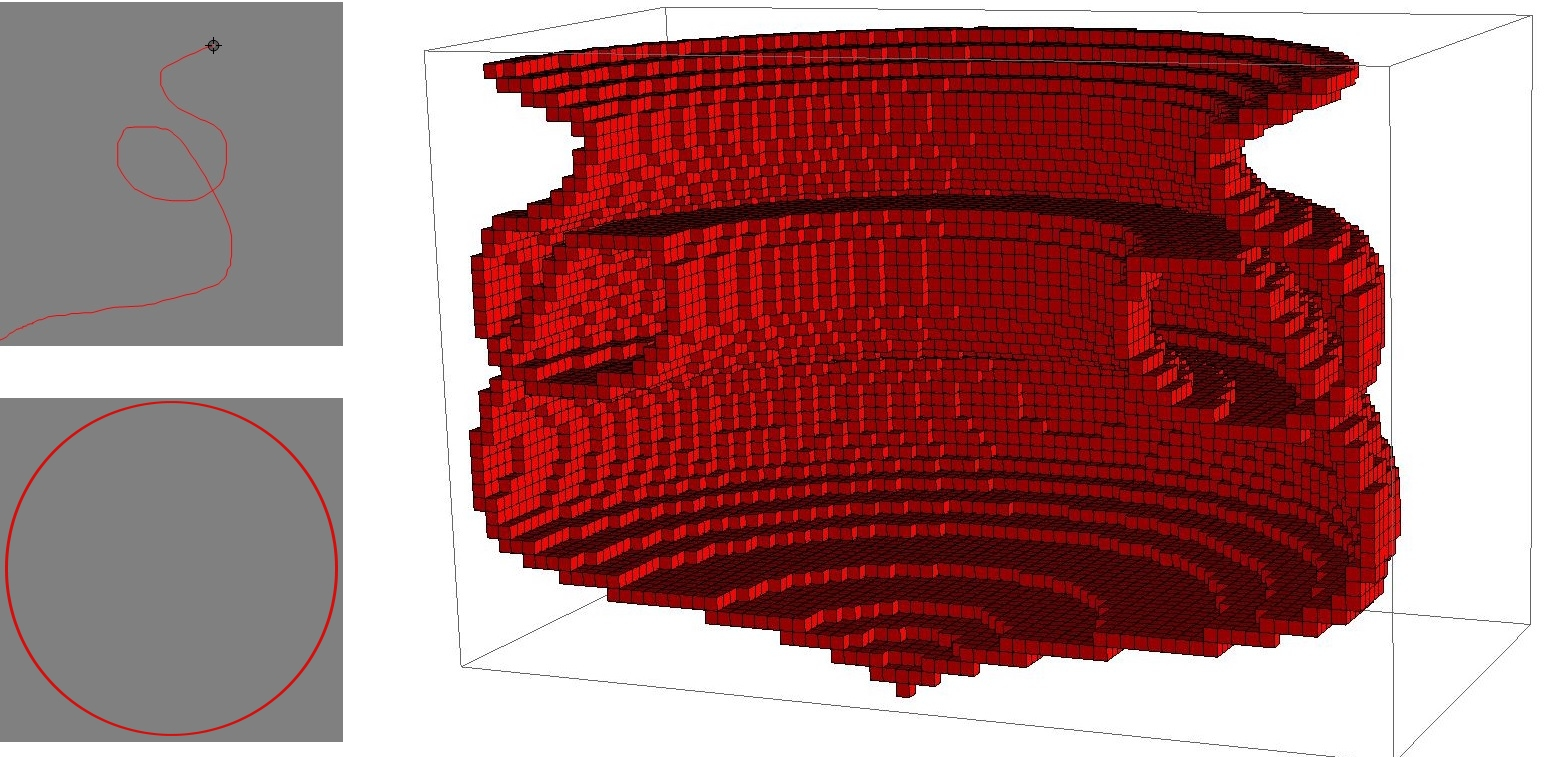
\includegraphics[height=3.8cm]{../Images/revolution2.jpg}
		\end{figure}
		\begin{itemize}
			\item The need is that tool have to be useable by everyone and everywhere
		\end{itemize}
	\end{frame}
	


%===============================================================================
%	ORGANISATION
%===============================================================================

\section{Staff Organization}


% --- Roles --------------------------------------------------------------------
	 \subsection{Roles}
	 \begin{frame}{\subsecname}
		\begin{itemize}
			\item Team composition~:
				\begin{itemize}
					\item Thomas \smallcaps{Benoist} - Project manager
					\item Zied \smallcaps{Ben} \smallcaps{Othmane} - Quality manager
					\item Adrien \smallcaps{Bisutti} - Risks manager
					\item Lydie \smallcaps{Richaume} - Tasks manager
				\end{itemize}
		\end{itemize}
	\end{frame}


% --- Réunion ------------------------------------------------------------------
	\subsection{Meetings}
	\begin{frame}{\subsecname}
		\begin{itemize}
			\item Milestone meetings :
			\begin{itemize}
				\item With the clients
				\item First meeting : around December 20th,2015
				\item Possibility to add meetings during the project
			\end{itemize}
			\item Audits
			\begin{itemize}
				\item In presence of the auditor, the clients and the pedagogic supervisor
				\item Followup meeting, Progress meeting, Delivery, Presentation
			\end{itemize}
			\item Meeting with the pedagogic supervisor every week
		\end{itemize}
	\end{frame}



%===============================================================================
%	DEROULEMENT
%===============================================================================

\section{Planification}


% --- Taches -------------------------------------------------------------------
	\subsection{Tasks}
	\begin{frame}{\subsecname}
		\begin{center}
		{\renewcommand{\arraystretch}{1.3}
		\begin{tabularx}{11cm}{|>{\hfill}X<{\hspace*{\fill}}|X<{\centering}|} % FIXME numéroter les tâches et faire voir les numéros le plus possibles !
			\hline
			\multicolumn{2}{|c|}{1 - Documentation, test et aide utilisateur}\\
			\hline
			\multicolumn{2}{|c|}{6 - Conception}\\
			\hline
			6 - Noyau fonctionnel & 10 - Interface minimale\\
			\hline
			17 - Ajout de fonctionnalités & \multirow{3}*{14, 22, 32 - Am\'elioration IHM}\\
			\cline{1-1}
			25 - M\'eridienne \`a main levée & \\%Am\'elioration IHM\\
			\cline{1-1}
			29 - Gestion des donn\'ees & \\%Am\'elioration IHM\\
			\hline
			\multicolumn{2}{|c|}{36 - Ajout courbe utilisateur}\\
			\hline
			\multicolumn{2}{|c|}{37 - R\'edaction rapport technique}\\
			\hline
		\end{tabularx}}
		\end{center}
	\end{frame}


% --- Pert ---------------------------------------------------------------------
	\subsection{Pert Diagram} % FIXME numéroter les tâches pour pouvoir utiliser cette numérotation
	\begin{frame}{Pert}
		\begin{figure}
			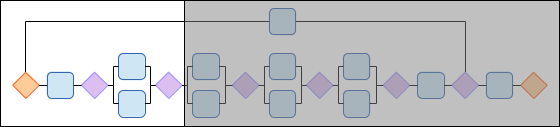
\includegraphics[width=6cm]{ImagesLancement/miniature1.png}
		\end{figure}\begin{figure}
			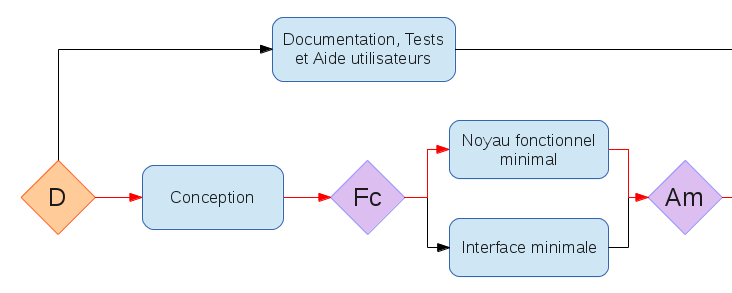
\includegraphics[width=11cm]{ImagesLancement/pert_part_1.png}
		\end{figure}
		\footnotesize{D~: Start (30/10) \hfill Am~: Minimal appli. (24/12) \\
			\hfill Fc~: End of design (16/12) \hspace*{\fill}}
	\end{frame}

	\begin{frame}{Pert}
		\begin{figure}
			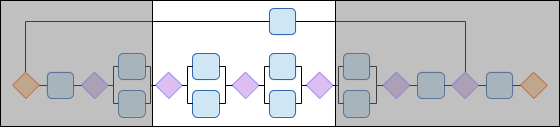
\includegraphics[width=6cm]{ImagesLancement/miniature2.png}
		\end{figure}\begin{figure}
			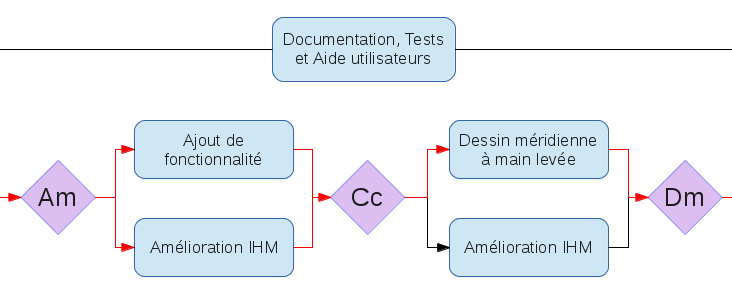
\includegraphics[width=11cm]{ImagesLancement/pert_part_2.png}
		\end{figure}
		\footnotesize{Am~: Minimal appli(24/12) \hfill Dm~: Hand free drawing (28/01)\\
			 \hfill Cc~: Courb choice(20/01) \hspace*{\fill}}
	\end{frame}

	\begin{frame}{Pert}
		\begin{figure}
			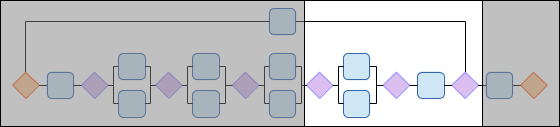
\includegraphics[width=6cm]{ImagesLancement/miniature3.png}
		\end{figure}\begin{figure}
			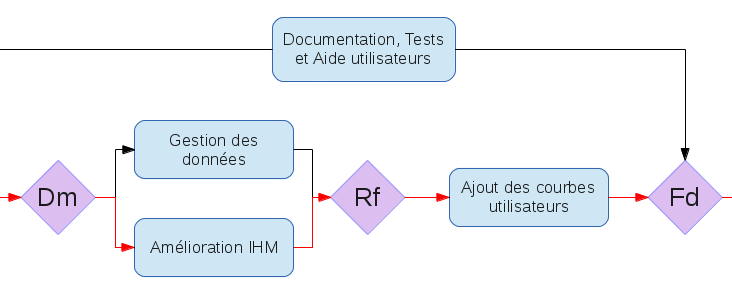
\includegraphics[width=11cm]{ImagesLancement/pert_part_3.png}
		\end{figure}
		\footnotesize{Dm~: Hand free drawing (28/01) \hfill Fd~: End of Development (02/03)\\
			 \hfill Rf~: Write formula (19/02)\hspace*{\fill}}
	\end{frame}

	\begin{frame}{Pert}
		\begin{figure}
			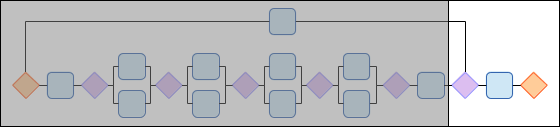
\includegraphics[width=6cm]{ImagesLancement/miniature4.png}
		\end{figure}\begin{figure}
			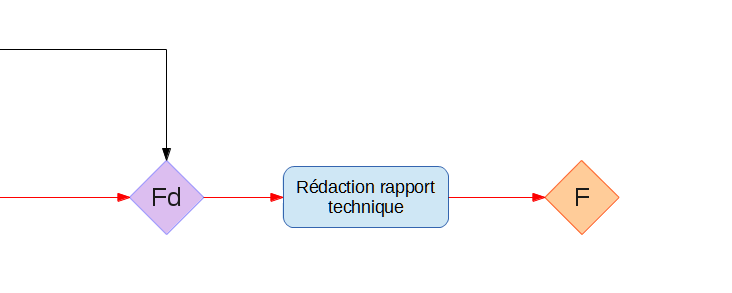
\includegraphics[width=11cm]{ImagesLancement/pert_part_4.png}
		\end{figure}
		\footnotesize{Fd~: End of Development (02/03) \hfill F~: Fin (17/03)\\[0.48cm]}
	\end{frame}
	

% --- Gantt --------------------------------------------------------------------
	\subsection{Gantt diagram}
	\begin{frame}{Gantt}
		\begin{figure}
			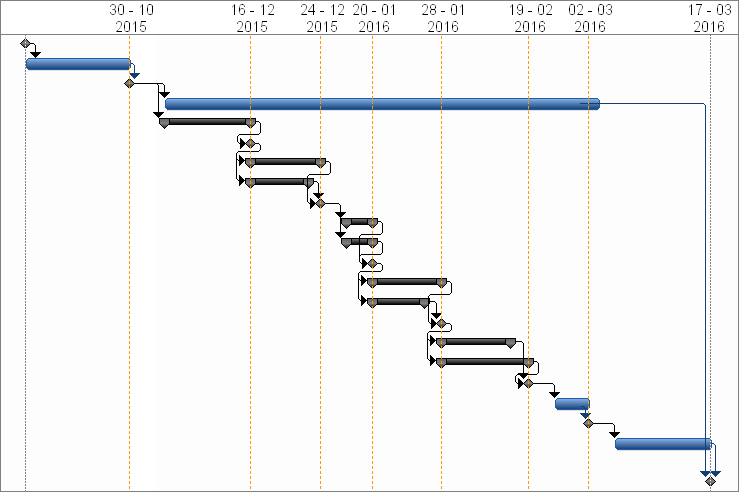
\includegraphics[height=7.5cm]{../Images/Gantt_Macro2.png} % FIXME mettre les tâches (nom et/ou numérotation) près des bandes
		\end{figure}
	\end{frame}


	\begin{frame}{Gantt}
		\begin{figure}
			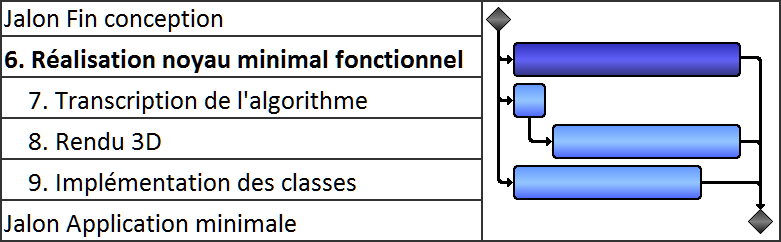
\includegraphics[width=12cm]{../Images/gantt_zoom_noyau.png} % FIXME modifier nom jalon
		\end{figure}
	\end{frame}


% --- Avancement ---------------------------------------------------------------
	\subsection{Progress}
	\begin{frame}{\subsecname}
		\begin{figure}
			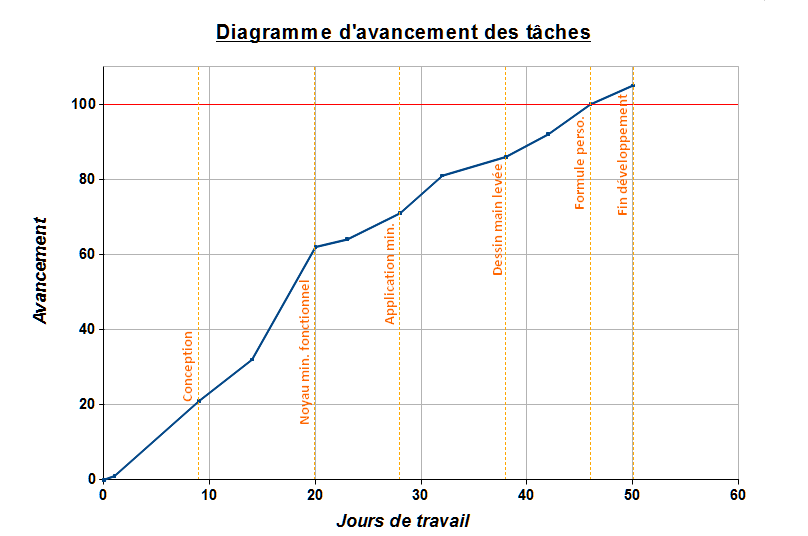
\includegraphics[width=12cm]{ImagesLancement/Avancement.png} % FIXME bien régler les points et faire apparaitre le livrables
		\end{figure}
	\end{frame}


% --- Livrables ----------------------------------------------------------------
	\subsection{Deliverables}
	\begin{frame}{\subsecname}
		\begin{center}
		{\renewcommand{\arraystretch}{1.2}
		\begin{tabular}{|c|m{6.5cm}|c|} % FIXME relier les livrables au tâches
			\hline
			\textbf{\No} & \textbf{Deliverable} & \textbf{Planned date}\\
			\hline
			1 & Interface and algorithm result & 12/23\\
			\hline
			2 & Minimal application & 01/21\\
			\hline
			3 & Free Hand drawing and curves with editable parameters & 01/29\\
			\hline
			4 & \'Equations and export & 02/19\\
			\hline
			5 & Final application and documentation & 03/02\\
			\hline
		\end{tabular}}
		\end{center}
		Deliverables types~:
		\begin{itemize}
			\item Software version~: all
			\item User documentation~: all
			\item Technical documentation~: 1 and 5
		\end{itemize}
	\end{frame}



%===============================================================================
%	RISQUES
%===============================================================================

\section{Risks}


% --- Risques ------------------------------------------------------------------
	\subsection{Specifics Risks}
	\begin{frame}{\subsecname}
		List of identified risks~:
			\begin{itemize}
				\item Generation of evolution algorithm (criticality~: 2)
				\item Difficulty to transcript the algorithm (Mathematica $\to$ Javascript) (1)
				\item Interface will be developed for two types of users (1)
				\item 3D Rendering using too much resources (1)
				\item Server linked problems (0)
			\end{itemize}
	\end{frame}

% FIXME ne pas oublier les solution (préventives et curatives) au moins à l'oral
	\begin{frame}{\subsecname}
		\begin{itemize}
			\item Evolution of the generation algorithm
		\end{itemize}
		\begin{figure}
			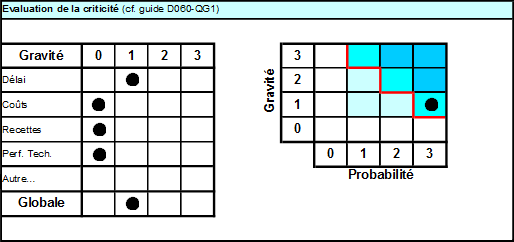
\includegraphics[width=8cm]{ImagesLancement/Evolution_algo.png}
		\end{figure}
		\begin{figure}
			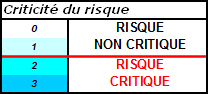
\includegraphics[height=2cm]{ImagesLancement/legende_risque2.png} % FIXME compléter avec légende gravité et probabilité
		\end{figure}
	\end{frame}

	\begin{frame}{\subsecname}
		\begin{itemize}
			\item Interface will be developed for two types of users
		\end{itemize}
		\begin{figure}
			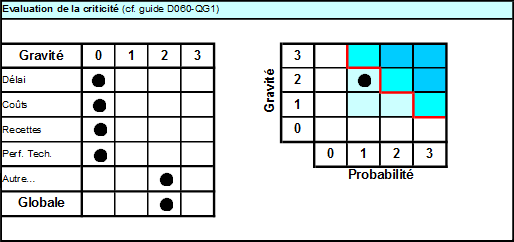
\includegraphics[width=8cm]{ImagesLancement/Interface_2_user.png}
		\end{figure}
		\begin{figure}
			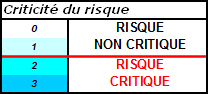
\includegraphics[height=2cm]{ImagesLancement/legende_risque2.png} % FIXME compléter avec légende gravité et probabilité
		\end{figure}
	\end{frame}


	\begin{frame}{\subsecname}
		\begin{itemize}
			\item Problems related to the server
		\end{itemize}
		\begin{figure}
			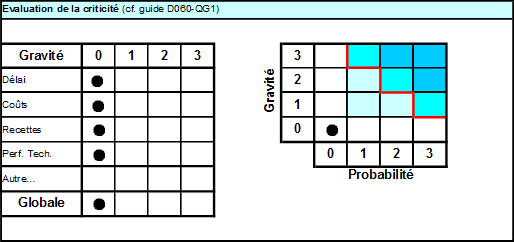
\includegraphics[width=8cm]{ImagesLancement/Serveur.png}
		\end{figure}
		\begin{figure}
			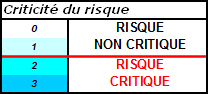
\includegraphics[height=2cm]{ImagesLancement/legende_risque2.png} % FIXME compléter avec légende gravité et probabilité
		\end{figure}
	\end{frame}


% --- Risques génériques -------------------------------------------------------
	\subsection{Generic risks}
	\begin{frame}{\subsecname}
		\begin{itemize}
			\item New clients (criticality~: 1)
			\item Non-compliance of the requirements (1)
			\item Non usability of tools (1)
			\item insufficient intern communication (1)
		\end{itemize}
	\end{frame}



%===============================================================================
%	MISE EN OEUVRE ÉQUIPE
%===============================================================================

\section{Methodology}


% --- Mise en oeuvre -----------------------------------------------------------
	\subsection{Application}
	\begin{frame}{\subsecname}
		\begin{itemize}
			\item Spiral development
				\begin{itemize}
					\item Deliverable for every developments cycles (Software version and documentation associated)
					\item Documentation and tests during every developments cycles
					\item Adaptation to the client requests
					\item Six developments cycles
				\end{itemize}
		\end{itemize}
		\begin{itemize}
			\item Quality insurance plan
				\begin{itemize}
					\item QIP~: ISO-9126 standard
 					\item Given a quality note according to different criteria
					\item internal and external tests
				\end{itemize}
		\end{itemize}
	\end{frame}


% --- Tests --------------------------------------------------------------------
	\subsection{Tests}
	\begin{frame}{\subsecname}
		\begin{block}{Internal tests}
			\begin{itemize}
				\item Quality code mesurment
				\item Tests plan defined by the quality manager
				\item Unit tests conducted by the developers
				\item Integration tests conducted by the quality manager
			\end{itemize}
		\end{block}

		\begin{block}{External tests}
			\begin{itemize}
				\item Validation of the application by the clients and the quality manager
				\begin{itemize}
					\item Functionalities validation
					\item Interface validation
				\end{itemize}
				\item Quiz scripts given to the clients
			\end{itemize}
		\end{block}
	\end{frame}


% --- Tests --------------------------------------------------------------------
	\subsection{Quality insurance plan}
	\begin{frame}{\subsecname}
		\begin{figure}
			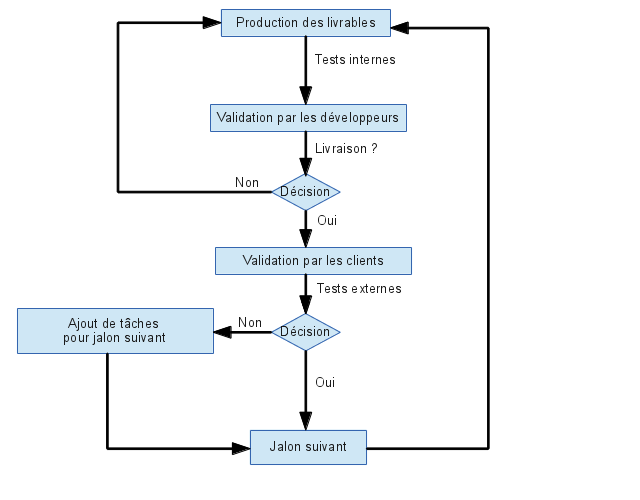
\includegraphics[height=8cm]{ImagesLancement/PAQL.png} % FIXME regénéré pour être plus lisible et spécifié "validation par les clients à chaque jalon"
		\end{figure}
	\end{frame}



%===============================================================================
%	COUTS
%===============================================================================

\section{Costs}


\begin{frame}{\secname}
	\begin{itemize}
		\item Project cost~:
			\begin{itemize}
				\item Junior engineer~: 3 000 \Euro{} / month
				\item 4 persons during 10 weeks
				\item Cost price~: 30 000 \Euro 
				\item Selling price proposed~: 40 000 \Euro
			\end{itemize}
	\end{itemize}
	\begin{itemize}
		\item Distribution of payments~:
			\begin{itemize}
				\item 30\% \`when the requirements are signed (12 000 \Euro)
				\item 10\% for every deliverables (4 000 \Euro)
				\item 30\% \`for the final delivery
			\end{itemize}
	\end{itemize}
\end{frame}


\begin{frame}{\secname}
	\begin{figure}
		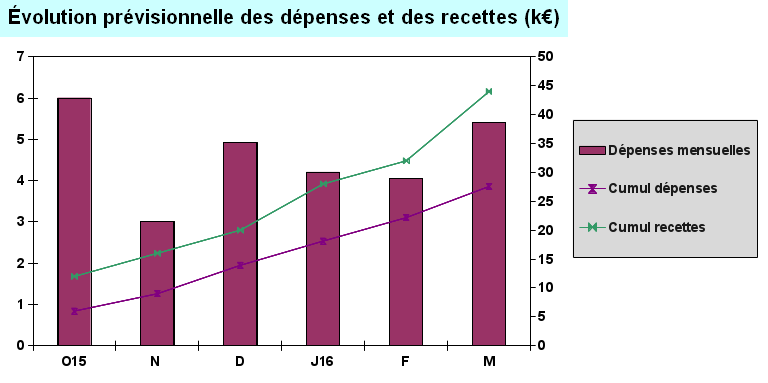
\includegraphics[width=12cm]{ImagesLancement/Cout2.png} % XXX voir ce que ça donne en semaine
	\end{figure}
\end{frame}



%===============================================================================
%	CONCLUSION
%===============================================================================

\section{Conclusion}


% --- Rappel -------------------------------------------------------------------
\begin{frame}{\secname}
	\begin{itemize}
		\item Cycles organization $\to$ incremental developpement
		\item Consistent validation with the clients
		\item Only one critical risk
		\item Next milestone~: Design phase
	\end{itemize}
\end{frame}


% --- Remerciment --------------------------------------------------------------
\begin{frame}{}
	\bigskip
	\bigskip
	\begin{titleblock}{}
		\begin{center}
			\smallskip
			\Large Discrete surfaces of revolution\\
			\medskip
			\small English presentation
			\smallskip
		\end{center}
	\end{titleblock}

	\bigskip
	\begin{center}
		Thanks for your attention.\\
		\medskip
		Are there any questions\,?			
	\end{center}

	\bigskip
	\bigskip
	
\includegraphics[width=2cm]{../Images/logo-Xlim.png}
	\hfill
	
\includegraphics[width=2cm]{../Images/logo_univ_poitiers.png}
\end{frame}


\end{document}


